\usetikzlibrary{calc}
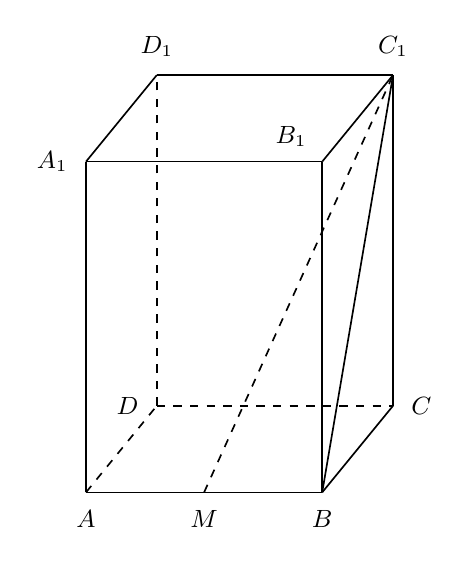
\begin{tikzpicture}[line width=.6pt, font=\small, x=1cm, y=1cm]
\coordinate (A) at (0,0);
\coordinate (M) at (1.5,0);
\coordinate (B) at (3,0);
\coordinate (D) at (0.9,1.1);
\coordinate (C) at (3.9,1.1);
\coordinate (A1) at (0,4.2);
\coordinate (B1) at (3,4.2);
\coordinate (D1) at (0.9,5.3);
\coordinate (C1) at (3.9,5.3);
% visible solids
\draw (A)--(B);
\draw (A)--(A1);
\draw (B)--(B1);
\draw (B)--(C);
\draw (C)--(C1);
\draw (A1)--(B1);
\draw (D1)--(C1);
\draw (A1)--(D1);
\draw (B1)--(C1);
\draw (B)--(C1);
% hidden dashed
\draw[dashed] (A)--(D);
\draw[dashed] (D)--(C);
\draw[dashed] (D)--(D1);
\draw[dashed] (M)--(C1);
% labels offset to avoid strokes
\node[below=3pt] at (A) {$A$};
\node[below=3pt] at (M) {$M$};
\node[below=3pt] at (B) {$B$};
\node[left=3pt] at (D) {$D$};
\node[right=3pt] at (C) {$C$};
\node[left=3pt] at (A1) {$A_{1}$};
\node[above left=2pt] at (B1) {$B_{1}$};
\node[above=3pt] at (D1) {$D_{1}$};
\node[above=3pt] at (C1) {$C_{1}$};
\end{tikzpicture}
